%\documentclass{article}
%
%\usepackage[spanish]{babel}
%\usepackage[utf8]{inputenc}
%\usepackage{geometry}
%\usepackage{graphicx}
%\geometry{tmargin=3cm,bmargin=3cm,lmargin=3cm,rmargin=2cm}
%
%\begin{document}

\setlength{\unitlength}{1cm}
%\begin{picture}(17,21)
%\put(0,0) {\line(1,0){17}}
%\put(0,21) {\line(1,0){17}}
%\put(0,21) {\line(0,-1){21}}
%\put(17,21) {\line(0,-1){21}}
%\end{picture}

\begin{picture}(17,21)
\put(8,4)
{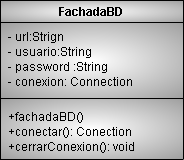
\includegraphics[width=5cm, height=4cm]{DiagramasClase/Utilidades}}
\put(0,2)
{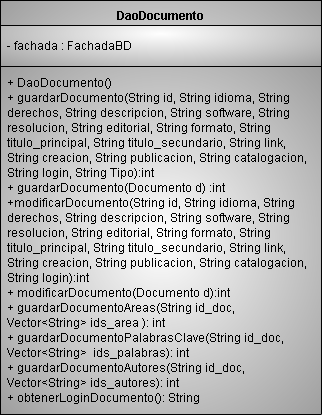
\includegraphics[width=7cm, height=10cm]{DiagramasClase/Documentos/DaoDocumento}}
\put(8,9)
{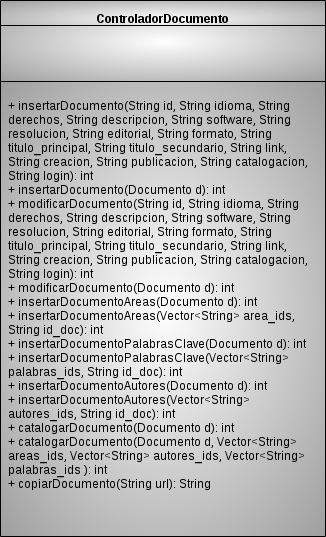
\includegraphics[width=7cm, height=12cm]{DiagramasClase/Documentos/ControladorDocumento}}
\put(0,13)
{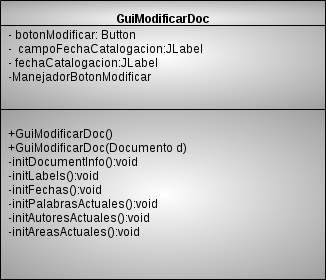
\includegraphics[width=7cm, height=8cm]{DiagramasClase/Documentos/GuiModificarDoc}}
\end{picture}


\newpage

\begin{picture}(17,21)
\put(0,0)
{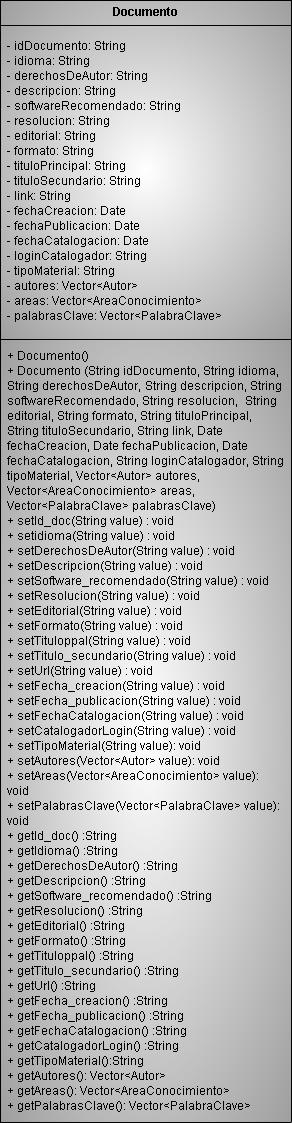
\includegraphics[width=7cm, height=21cm]{DiagramasClase/Documentos/Documento}}
\put(8,-1)
{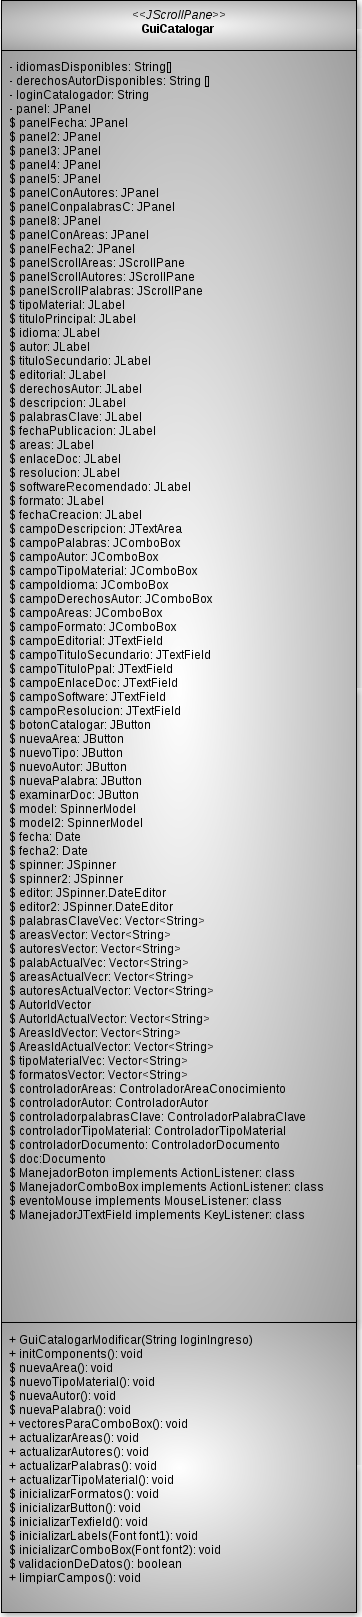
\includegraphics[width=8cm, height=22cm]{DiagramasClase/Documentos/GuiCatalogar}}
\end{picture}

%\end{document}